\section{Architekturübersicht}
\label{kap:Architek}
Nach der Vorstellung der verwendeten Technologien beschreibt dieser Abschnitt den Aufbau der Gesamtarchitektur. Für das Lesen der Arbeit stellt die Übersicht eine Orientierungshilfe dar, um die technische Gliederung der Lösung von Beginn an nachvollziehbar zu machen. Die nachfolgende Beschreibung orientiert sich an der nummerierten Abbildung~\ref{fig:architekturuebersicht}, um das Zusammenspiel der Komponenten sowie den Datenfluss übersichtlich darzustellen und nachvollziehbar zu machen.

Die entwickelte Lösung ist in drei Hauptbereiche unterteilt: (1) Datenbank, (2) Backend und (3) VS Code Extension.

Die Graphdatenbank (1) speichert die Entitäten der Anwendung und liest beim Start das definierte Datenbankschema (1.1) ein, welches deren Struktur, Typen und mögliche Beziehungen festlegt.

Im Backend (2) übernehmen zwei Controller die Kommunikation mit der Datenbank. Der VFS Controller (2.1) verarbeitet Anfragen des virtuellen Filesystems. Der LSP Controller (2.2) liefert dem VFS Language Server (2.3) die Daten, welche dieser benötigt, um Anfragen des Editors für Validierung, Autocompletion und Go-to-Definition zu beantworten.

Innerhalb von Visual Studio Code (3) bestehen zwei Extensions mit getrennten Verantwortlichkeiten. Die Virtual Filesystem Extension (3.1) stellt eine Benutzeroberfläche im Explorer und im Editor bereit, über welche Datenobjekte navigiert sowie erstellt, geöffnet, bearbeitet und gespeichert werden können. Die VFS Language Client Extension (3.2) unterstützt den Editor mit Funktionen wie Validierung und Autovervollständigung. Die Aktivierung erfolgt beim Öffnen des Editors, wobei die Extension auf Aktionen wie das Bearbeiten von Dateien reagiert.

\begin{figure}[H]
    \centering
    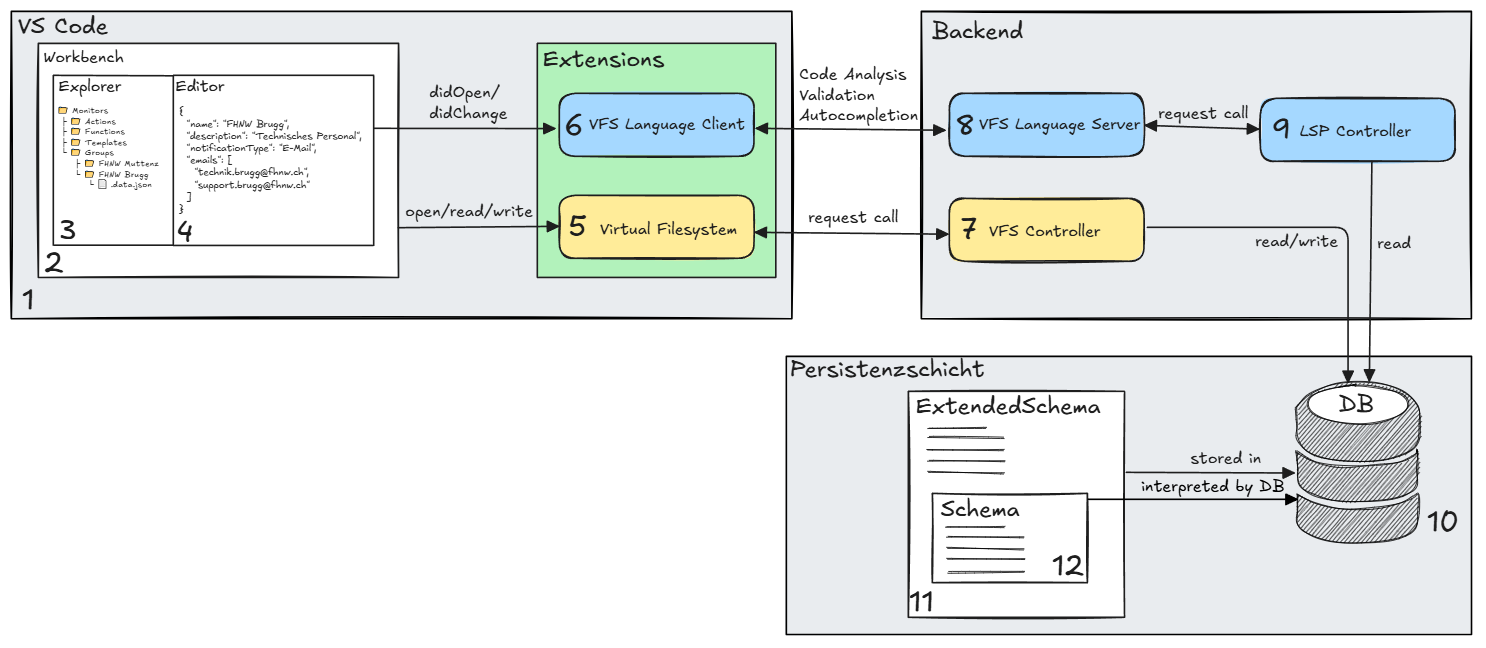
\includegraphics[width=1\linewidth]{arch.png}
    \caption{Architektur desMonidas Code Assist Navigator}
    \label{fig:architekturuebersicht}
\end{figure}
